\section{Week 3 - 28 Jan 2022 - Motion in wire and track}
First we will look at motion in 1D, and then find useful results to look in more
general systems -- bead on wire and track motion.
Note that for 1D motion, the vector equations of motion are really scalar.
Consider the motion given by 
\[\vec{F}=m\ddot{\vec{x}} \implies \dot{\vec{x}}\cdot\vec{F} =
m\dot{\vec{x}}\cdot\ddot{\vec{x}}\implies \dot{x}F=m\dot{x}\ddot{x}\]
\[\implies \frac{d}{dt}\left( \frac{1}{2}m\dot{x}^2 - \int_{x_0}^xF(s)ds
\right)=0\]
\[\therefore \frac{1}{m}v^2 + \phi = E\in\RR.\]
Where $E$ is a constant.
\begin{proposition}
  In $1D$ motion, forces are always conservative.
\end{proposition}
\begin{proof}
Observe that in $1D$, $\vec{F}=F\vec{e_x}$, so that $\nabla \times
F\vec{e_x}=0$.
\end{proof}

Next, the lecturer puts an example of 1D particle-in-a-potential-well problem,
to find that, from energy conservation, motion will be constrained to potential
energy that cannot go over the initial potential, and finds an oscillating phase
portrait. However, I don't understand why $\phi=mx^2$ is a valid potential,
since it does not even have energy dimensions (there's no time).

\subsection{Motion on a smooth wire}
Picture a bead on a smooth wire, so that upon motion, the reaction force can
have any direction -- which is different from the case of motion on track, which
can only have upward reaction force. In this setup, the reaction force $\vec{R}$
is always perpendicular to $\dot{\vec{x}}$, since $\vec{R}$ must be
perpendicular to the tangent of the wire. Hence $\vec{R}$ does not work. The
only other force acting on the bead is gravity, which is a conservative force.
Hence, energy conservation holds,
\[\frac{1}{2}mv^2 + \phi = E\in\RR.\]
Consider the wire to be described parametrically by $\vec{X}(s)$ for
$s=s(t)\in[s_0,s_1]$, where $t$ is the free variable. Hence the location of the
bead at time $t$ is $\vec{x}(t)=\vec{X}(s(t))$, and using the chainrule
\[\dot{\vec{x}} = \dot{s} \vec{X}'.\]
Where $\vec{X}'$ is the derivative wrt s -- recall that dot-notation is reserved
for time-derivatives. For gravity, the potential is given by
$\phi=m\vec{g}\cdot\vec{x}$. Therefore conservation of energy expands to
\[\frac{1}{2}m\dot{s}^2 |\vec{X}'|^2 + m\vec{g}\cdot\vec{X}(s(t)) = E.\]
Let us define $V=\frac{1}{m}\phi$, and let us use a parametrisation s.t.
$|\vec{X}'|=1$ (e.g. s is the arc length -- what does this mean?), so that we
can rewrite
\[\frac{1}{2}\dot{s}^2 + V = E/m.\]
This equation determines motion. \todo{Lecturer says $V$ depends on the path --
why? It's a potential, it shouldn't.}

\subsection{Motion on a track}
\begin{figure}[h]
  \centering
  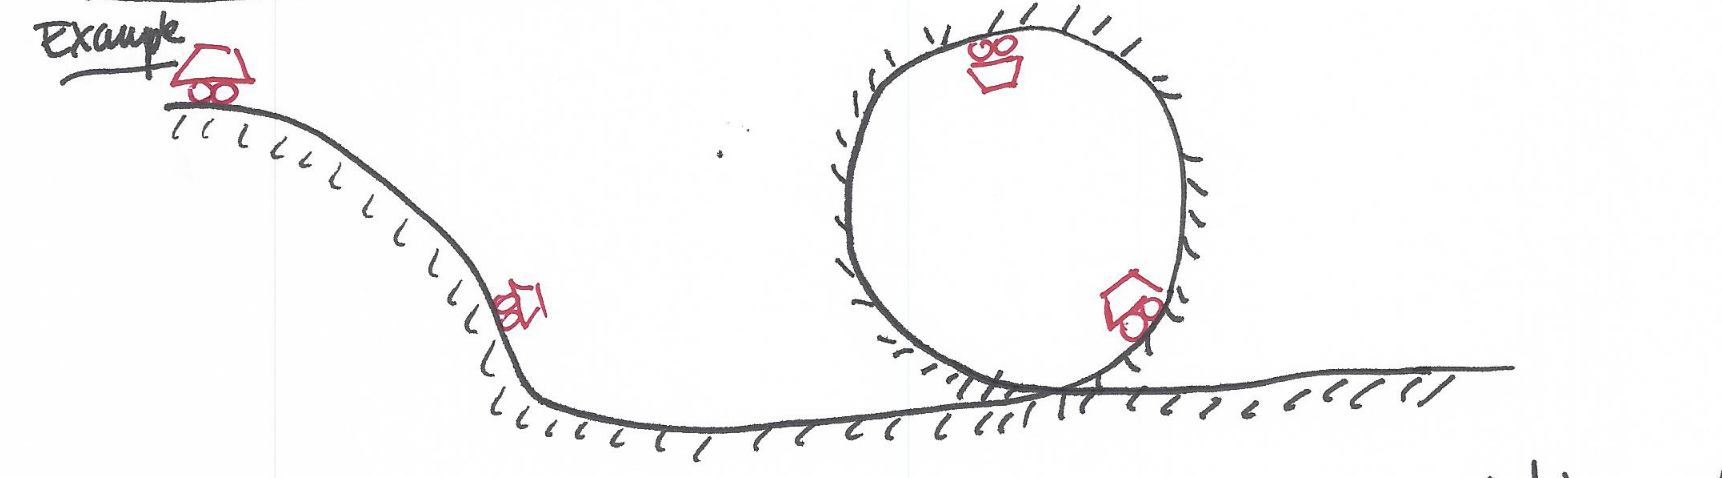
\includegraphics[width=\textwidth]{media/lec9_example}
  \caption{Example set up for motion on a track. Work of the Lecturer.}
  \label{fig:lec9_track_example}
\end{figure}
Consider the motion of a car as in the figure above. We want to figure out under
what conditions does the car stay complete the loop and doesn't fall down. In
other words, we want to find when the reaction is positive when the car is at
the top of the loop. Note that for motion on a track, the reaction force can
only be positive -- it can only push, not pull. We can reformulate the question
and look into when the car loses contact. That happens precisely when
$\vec{R}=\vec{0}$.

Consider the motion in the loop, where we can describe the motion with polar
coordinates, where $r=a$ is the radius of the loop, and $\theta$ is the angle
made at time $t$ -- when the car enters the loop, $\theta=0$, and when the car
reaches he top, $\theta=\pi$. Assuming that during the loop the car is in
contact with the track, we have 
\[\vec{x}=a\vec{e_r},\]
\[\dot{\vec{x}}=a\dot{\theta}\vec{e_{\theta}},\]
\[\ddot{\vec{x}} = a(\ddot{\theta}\vec{e_{\theta}} - \dot{\theta}^2\vec{e_r}).\]
We can consider the equation of forces,
\[\vec{F}=m\ddot{\vec{x}} = m\vec{g}+\vec{R}\]
\[ma(\ddot{\theta}\vec{e_{\theta}} - \dot{\theta}^2\vec{e_r})=
m\vec{g}-R\vec{e_r}.\]
We can take the dot product with $\vec{e_r}$ and find, 
\[-ma\dot{\theta}^2 = m\vec{g}\cdot\vec{e_r} - R=mg\cos(\theta) - R.\]
With the above data we can find the conservation of energy in the loop,
\[\frac{1}{2}ma^2\dot{\theta}^2 - mga\cos\theta = E\in\RR,\]
And use ICs to find $E$,
\[E=\frac{1}{2}mv_0^2 - mga.\]
Where $v_0$ is the initial speed when the car enters the loop, i.e. when
$\theta=0$ (hence $\cos(\theta)=1$). Equating
\[\frac{1}{2}mv_0^2 - mga = \frac{1}{2}ma^2\dot{\theta}^2 - mga\cos\theta\]
\begin{equation}
  \implies a\dot{\theta}^2 = \frac{v_0^2}{a}+2g(\cos\theta - 1).
  \label{eqn:lec9_example_track_theta}
\end{equation}

We can use this to help us with the expression for $R$,
\begin{equation}
  R = mg\cos\theta +ma\dot{\theta}^2 = m\left[ \frac{v_0^2}{a}+3g\cos\theta -2g
  \right].
  \label{eqn:lec9_example_track_R}
\end{equation}
We next ask when do $\dot{\theta}=0$ and when $R=0$. The first one is when the
car changes direction of motion, and the second one when the car loses contact
with the track. 
\todo{Ask the lecturer why does $\dot{\theta}=0$ implies that the car changes
direction?} Note that 
\[\dot{\theta}=0 \iff -\cos\theta= \frac{v_0^2}{2ag}-1,\]
\[R=0 \iff -\cos\theta = \frac{v_0^2}{3ag}-\frac{2}{3}.\]
Let us define $\xi=\frac{v_0^2}{ag}$, which will represent a variable defining
initial conditions (depends entirely on initial speed). Moreover, let us define
$\eta=-\cos\theta$. Observe then that the above equations really describe two
lines in $(\eta,\xi)$-space,
\todo{I don't understand how $\eta,\xi$ relate -- $\xi$ depends on ICs, but
$\eta$ changes along the loop, independent of ICs.}
\[\eta=\frac{1}{2}\xi -1,\]
\[\eta=\frac{1}{3}\xi -\frac{2}{3}.\]
We can plot this in a $(\eta,\xi)$ plane, as in Figure
\ref{fig:lec9_example_regime}.
\begin{figure}[h]
  \centering
  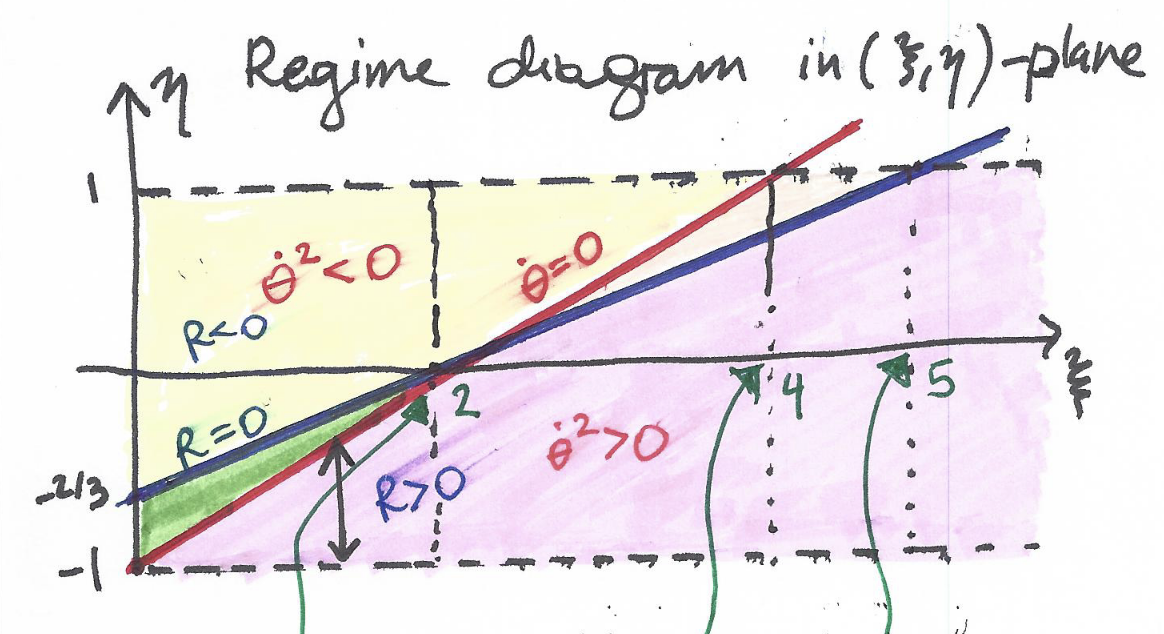
\includegraphics[width=\textwidth]{media/lec9_example_regime}
  \caption{Regime diagram of $(\xi,\eta)$-plane. The colors represent different
  configurations of $\dot{\theta}$ and $R$. Work of the Lecturer.}
  \label{fig:lec9_example_regime}
\end{figure}
Note that when $\theta=\pi$, $\eta=-\cos\theta=1$ and when $\theta=0,2\pi$,
$\eta=-1$. That's why $\eta\in[-1,1]$. Note that when $\dot{\theta}^2<0$ we have
$\eta>\frac{1}{2}\xi-1$ (think about Equation
\ref{eqn:lec9_example_track_theta}, and what does it mean for
$\dot{\theta}^2<0$). Obviously this is an impossible scenario (that would give
$\dot{\theta}\in\CC$ with non-zero imaginary part). On the other hand, when
$R<0$, then by looking at Equation \ref{eqn:lec9_example_track_theta} we observe
that this corresponds to $\eta>\frac{1}{2}\eta -2/3$. The opposite is true for
$\dot{\theta}^2>0, R>0$. The colors hence represent the following
\begin{enumerate}
  \item Yellow: $\dot{\theta}^2<0, R<0$ -- impossible.
  \item Green: $\dot{\theta}^2 <0, R>0$ -- impossible.
  \item Orange: $\dot{\theta}^2>0, R<0$ -- Loses contact with track.
  \item Pink: $\dot{\theta}^2>0, R>0$ -- In contact with track, completes loop.
\end{enumerate}
\todo{Ask lecturer about how does the evolution happen, as the car loops: is it
a vertical up and down along some IC $\xi$?} Observe how in Figure
\ref{fig:lec9_example_regime} we find the values of $\xi$ for which we find
$\eta=1$ and $\eta=0$-incerpects. We now ask what are the physical
interpretations of this solution,
\begin{enumerate}
  \item $\xi\geq 5$: Only pink region is possible, hence the car performs a
    loop.
  \item $\xi\leq 2$: Since pink region is the only possible one situation, the
    car will still perform a ``loop'' but with $\eta$ bounded, that is, with
    $\theta$ bounded -- it will oscillates between two turning points. Think of
    letting a skate board go in a ramp, it just oscillates like a pendulum.
  \item $\xi\in [2,5]$: The orange region is reached, so that when this happens,
    that is when $\theta$ reaches that angle, the car will fall
\end{enumerate}

